\documentclass[12pt]{article}
\usepackage[paperwidth=56in,paperheight=56in,margin=0.8in]{geometry}
\usepackage[T1]{fontenc}
\usepackage{helvet}
\renewcommand{\familydefault}{\sfdefault}
\usepackage{graphicx}
\usepackage{booktabs}
\usepackage{array}
\usepackage{xcolor}
\usepackage[most]{tcolorbox}
\usepackage{tikz}
\usetikzlibrary{positioning,arrows.meta}
\usepackage{enumitem}
\setlist[itemize]{leftmargin=1.0em,itemsep=0.25em,topsep=0.2em}
\pagestyle{empty}
\setlength{\parindent}{0pt}
\setlength{\parskip}{0.35em}

\definecolor{headerbg}{RGB}{24,75,120}
\definecolor{boxborder}{RGB}{35,85,130}
\definecolor{boxbg}{RGB}{247,250,253}
\definecolor{accent}{RGB}{192,57,43}
\definecolor{chipbg}{RGB}{232,241,249}

\newtcolorbox{posterbox}[2][]{
  enhanced,
  colback=boxbg,
  colframe=boxborder,
  coltitle=white,
  colbacktitle=boxborder,
  fonttitle=\bfseries\fontsize{44}{48}\selectfont,
  title=#2,
  boxrule=2pt,
  arc=8pt,
  left=16pt,
  right=16pt,
  top=12pt,
  bottom=10pt,
  valign=top,
  #1
}

\newcommand{\chip}[1]{%
  \tcbox[colback=chipbg,colframe=boxborder,arc=4pt,boxrule=1.2pt,left=6pt,right=6pt,top=3pt,bottom=3pt]{\Large\textbf{#1}}%
}

\newlength{\rowoneheight}
\newlength{\rowtwoheight}
\newlength{\rowthreeheight}
\setlength{\rowoneheight}{14.2in}
\setlength{\rowtwoheight}{20.0in}
\setlength{\rowthreeheight}{8.8in}

\begin{document}
\fontsize{30}{36}\selectfont

% Header
\begin{tcolorbox}[
  enhanced,
  colback=headerbg,
  colframe=headerbg,
  boxrule=0pt,
  arc=10pt,
  left=22pt,right=22pt,top=18pt,bottom=18pt,
  height=5.6in,
  valign=center
]
{\color{white}\fontsize{62}{68}\selectfont\textbf{MemoryAD: Training-Free Continual Anomaly Detection with Adaptive Coreset Memory}}\\[6pt]
{\color{white}\fontsize{36}{42}\selectfont Architecture-Agnostic Continual AD for Industrial Inspection}\\[10pt]
{\color{white}\fontsize{28}{34}\selectfont Team: [TO BE FILLED] \hfill Guide: [TO BE FILLED] \hfill Project ID: [TO BE FILLED] \hfill Department/Session: [TO BE FILLED]}
\end{tcolorbox}

\vspace{0.35cm}

% Row 1
\begin{minipage}[t][\rowoneheight][t]{0.318\textwidth}
\begin{posterbox}[height=\rowoneheight]{Introduction}
Industrial anomaly detection learns normal patterns to flag defects. In real factories, new product categories arrive sequentially, so the system must adapt without retraining on all previous categories. Standard continual-learning approaches often forget early categories after new updates. \textbf{MemoryAD avoids this by design: it does not update model weights and keeps old knowledge in a managed memory bank.}

\begin{center}
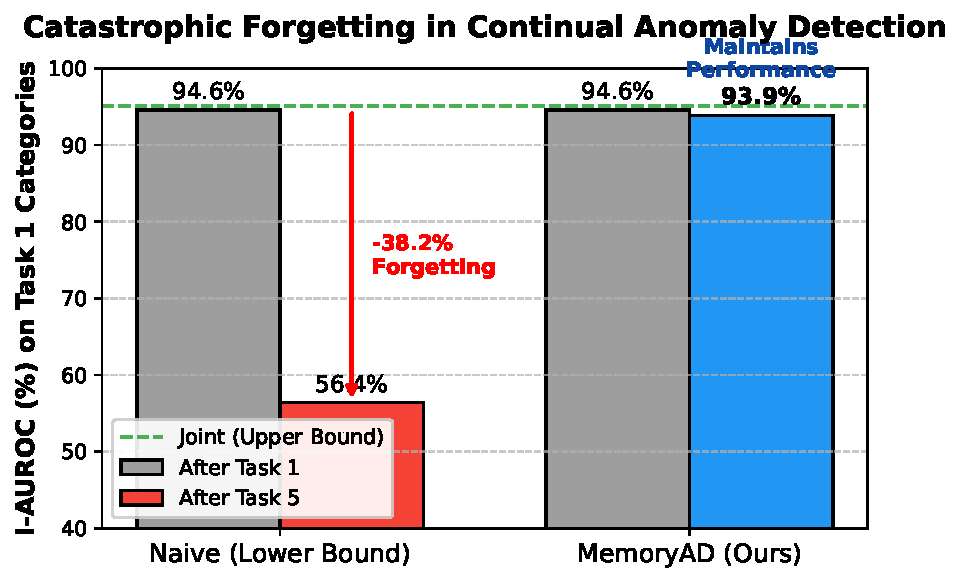
\includegraphics[width=0.93\linewidth]{../figures/f1_teaser.pdf}
\end{center}
\textbf{Message at a glance:} retraining-heavy continual methods degrade; MemoryAD stays stable through memory management.
\end{posterbox}
\end{minipage}\hfill
\begin{minipage}[t][\rowoneheight][t]{0.318\textwidth}
\begin{posterbox}[height=\rowoneheight]{Literature Survey}
\begin{itemize}
\item \textbf{Conventional AD:} PatchCore, PaDiM, EfficientAD, RD4AD are effective in static settings but do not directly solve category-incremental updates.
\item \textbf{Continual learning methods:} EWC, LwF, replay are designed for trainable classification models with parameter regularization.
\item \textbf{Gap for AD:} anomaly detection relies on modeling normality, so weight-regularization pipelines add complexity and still forget. MemoryAD keeps feature extraction frozen and manages memory instead.
\end{itemize}
\end{posterbox}
\end{minipage}\hfill
\begin{minipage}[t][\rowoneheight][t]{0.318\textwidth}
\begin{posterbox}[height=\rowoneheight]{Problem Definition and Objectives}
\textbf{Problem:} tasks $\mathcal{T}_1,\dots,\mathcal{T}_T$ arrive sequentially with normal-only training images from new categories. After each task, detect anomalies across all seen categories under fixed memory budget $B$.

\textbf{Project objectives}
\begin{itemize}
\item Adapt to new product categories incrementally.
\item Avoid retraining from scratch and avoid weight updates.
\item Keep memory bounded with global budget $B=10\text{K}$.
\item Minimize forgetting on earlier categories.
\item Evaluate on industrial benchmarks (MVTec AD, VisA).
\end{itemize}

\chip{Backbone: DINOv2 ViT-B/14}\hspace{0.25cm}
\chip{Layers: [7,11]}\hspace{0.25cm}
\chip{$k=9$}\hspace{0.25cm}
\chip{$B=10\text{K}$}
\end{posterbox}
\end{minipage}

\vspace{0.35cm}

% Row 2
\begin{minipage}[t][\rowtwoheight][t]{0.488\textwidth}
\begin{posterbox}[height=\rowtwoheight]{Model Architecture}
\begin{center}
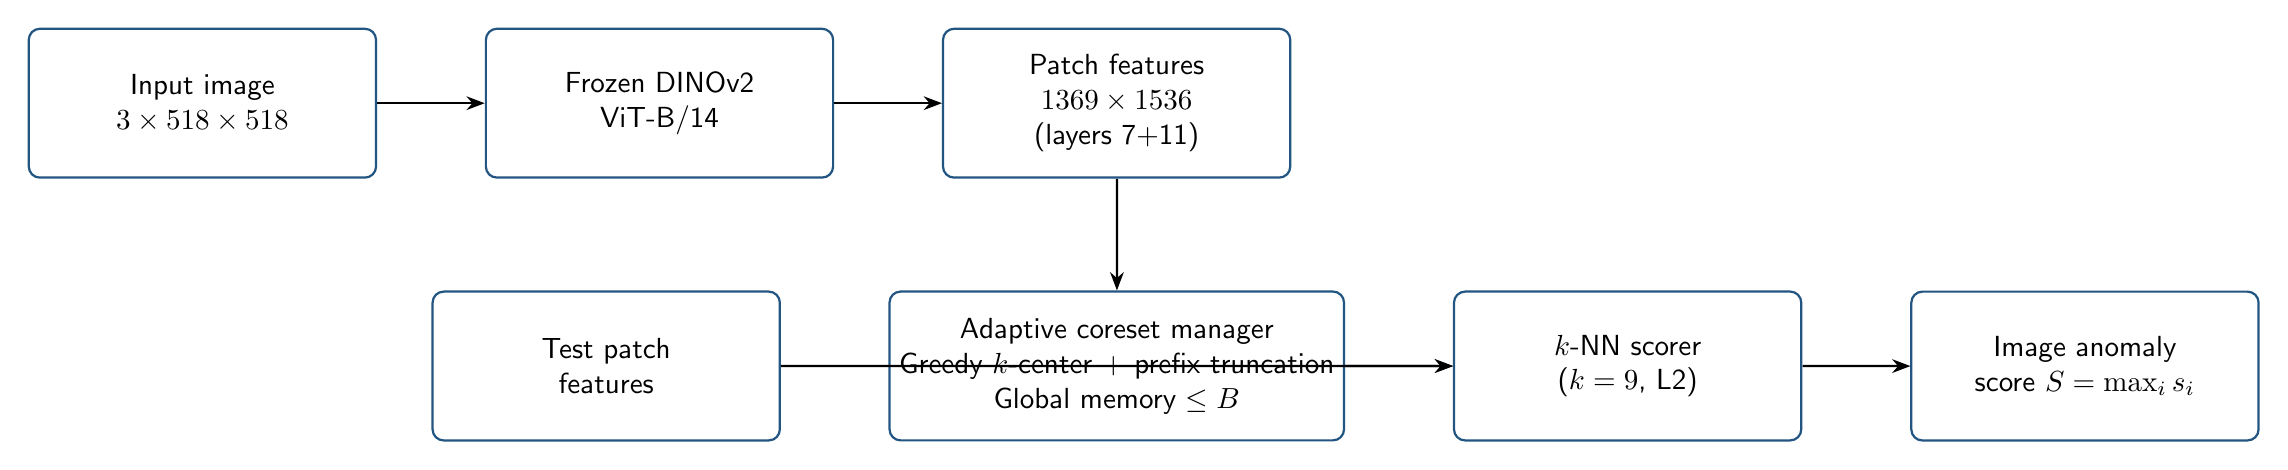
\begin{tikzpicture}[node distance=1.35cm, >=Stealth, scale=1.05, transform shape]
  \tikzstyle{blk}=[rectangle,rounded corners,draw=boxborder,thick,minimum width=4.2cm,minimum height=1.8cm,align=center,fill=white]
  \node[blk] (inp) {Input image\\$3\times 518\times 518$};
  \node[blk,right=1.3cm of inp] (dino) {Frozen DINOv2\\ViT-B/14};
  \node[blk,right=1.3cm of dino] (feat) {Patch features\\$1369\times1536$\\(layers 7+11)};

  \node[blk,below=1.35cm of feat,minimum width=5.4cm] (core) {Adaptive coreset manager\\Greedy $k$-center + prefix truncation\\Global memory $\leq B$};
  \node[blk,left=1.3cm of core] (test) {Test patch\\features};
  \node[blk,right=1.3cm of core] (knn) {$k$-NN scorer\\($k=9$, L2)};
  \node[blk,right=1.3cm of knn] (out) {Image anomaly\\score $S=\max_i s_i$};

  \draw[->,thick] (inp) -- (dino);
  \draw[->,thick] (dino) -- (feat);
  \draw[->,thick] (feat) -- (core);
  \draw[->,thick] (test) -- (knn);
  \draw[->,thick] (core) -- (knn);
  \draw[->,thick] (knn) -- (out);
\end{tikzpicture}
\end{center}

\textbf{Pipeline in code:}
\begin{itemize}
\item \texttt{src/pipeline.py}: task-wise update, coreset refresh, evaluate all seen categories.
\item \texttt{src/coreset/adaptive\_manager.py}: budget allocation and prefix truncation for old categories.
\item \texttt{configs/default.yaml}: default settings ($B=10\text{K}$, $k=9$, layers [7,11]).
\end{itemize}

\textbf{Core claim:} no model weight updates, so forgetting is driven mainly by controlled memory compression.
\end{posterbox}
\end{minipage}\hfill
\begin{minipage}[t][\rowtwoheight][t]{0.488\textwidth}
\begin{posterbox}[height=\rowtwoheight]{Results and Analysis}
\textbf{Main comparison (MVTec AD, 5-task)}
\begin{center}
\begin{tabular}{lcccc}
\toprule
Method & I-AUROC & FR & Avg Inc. & FT \\
\midrule
Joint (reference) & 95.1 & -- & -- & -- \\
\textbf{MemoryAD} & \textbf{94.0 $\pm$ 0.8} & \textbf{0.97} & \textbf{94.0} & \textbf{99.0} \\
Replay+RD4AD & 83.7 & -- & -- & -- \\
Naive & 78.4 & -- & -- & -- \\
EWC+RD4AD & 74.1 & -- & -- & -- \\
LwF+RD4AD & 70.0 & -- & -- & -- \\
\bottomrule
\end{tabular}
\end{center}

\begin{minipage}[t]{0.485\linewidth}
\centering
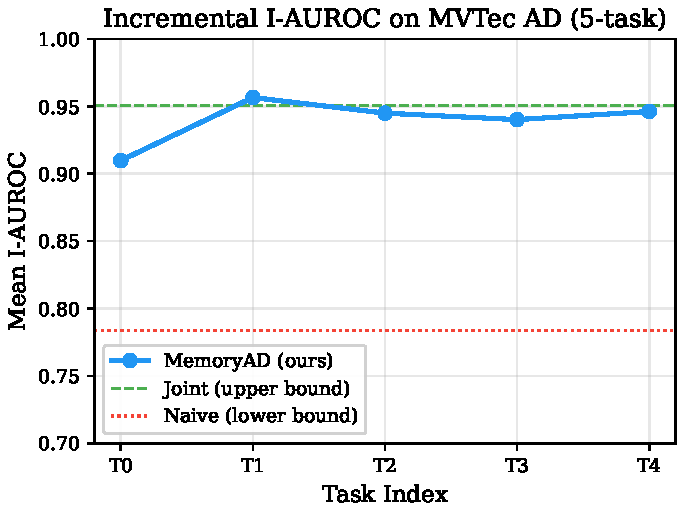
\includegraphics[width=\linewidth]{../figures/f2_incremental_auroc.pdf}\\[-2pt]
{\Large Stable incremental trend across tasks}
\end{minipage}\hfill
\begin{minipage}[t]{0.485\linewidth}
\centering
\includegraphics[width=\linewidth]{../figures/f7_qualitative_heatmaps.pdf}\\[-2pt]
{\Large Strong qualitative localization}
\end{minipage}

\vspace{0.4em}
\chip{VisA I-AUROC: 90.3}\hspace{0.2cm}
\chip{Throughput: 29.6 ms/image}\hspace{0.2cm}
\chip{Memory: 117.2 MB @ B=10K}
\end{posterbox}
\end{minipage}

\vspace{0.35cm}

% Row 3
\begin{posterbox}[height=\rowthreeheight]{Conclusion and Future Scope}
\begin{minipage}[t]{0.49\textwidth}
\textbf{Conclusion}
\begin{itemize}
\item MemoryAD combines frozen DINOv2 features, adaptive coreset memory, and k-NN scoring to deliver strong continual anomaly detection.
\item It achieves near-zero forgetting behavior in practice (FR=0.97 on MVTec AD) while avoiding retraining-heavy continual pipelines.
\end{itemize}
\end{minipage}\hfill
\begin{minipage}[t]{0.49\textwidth}
\textbf{Future scope}
\begin{itemize}
\item Improve fine-boundary localization with multi-scale feature fusion.
\item Extend to stronger domain-shift and domain-incremental scenarios.
\item Accelerate nearest-neighbor search for higher deployment throughput.
\end{itemize}
\end{minipage}
\end{posterbox}

\end{document}
